
\begin{frame}{Motivation}

Inferring population structure from genomic sequences.
\begin{itemize}
  \item[--] Genotype data \textit{Turdus helleri}, an endagered bird species
  {\color{blue} \href{https://web.stanford.edu/group/pritchardlab/publications/pdfs/PritchardEtAl00.pdf}{(Pritchard et al. 2011)}}.
  \item[--] Microsatellites sequences of 155 individiuals at 7 loci.
\end{itemize}


\begin{figure}[!h]
\centering
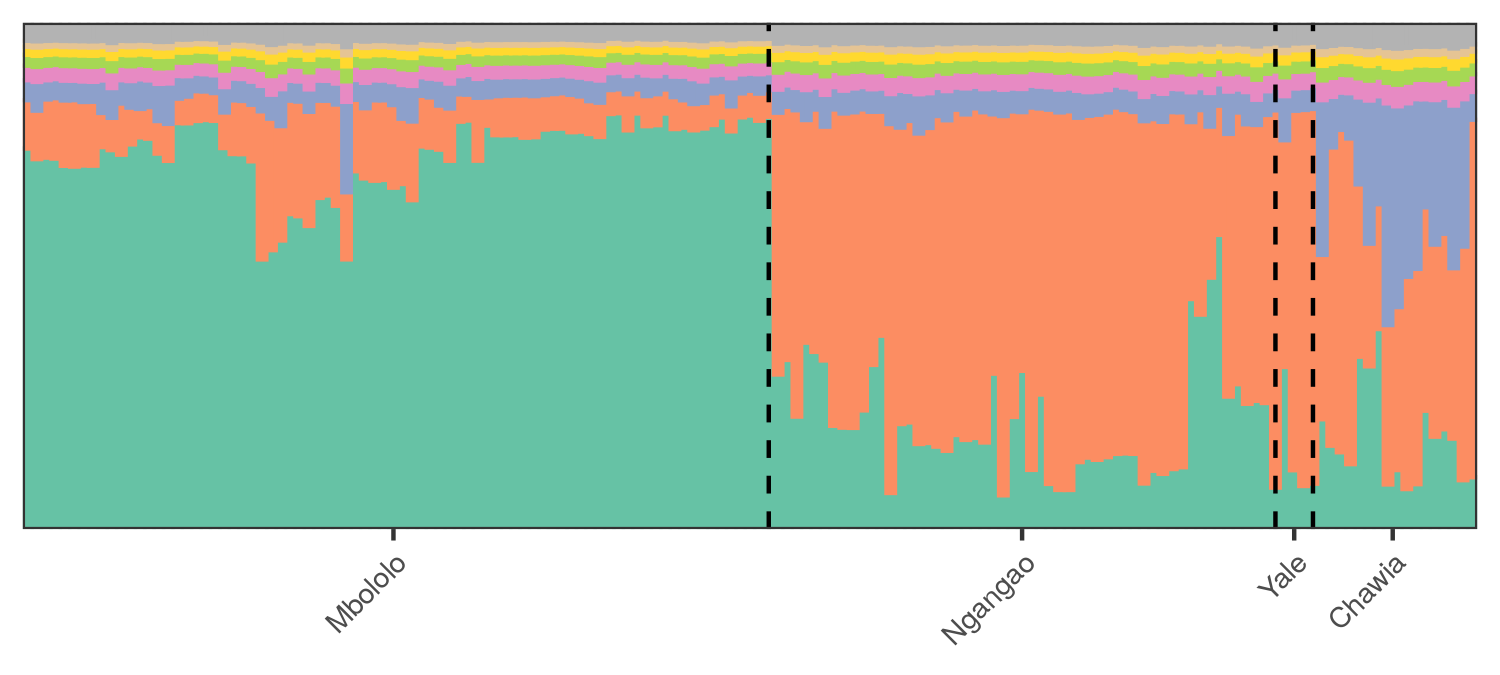
\includegraphics[width = 0.8\textwidth]{./figures/structure_example.png}
\end{figure}

\end{frame}

\begin{frame}{Motivation}

{\bf Scientific goal: } infer the number of ancestral populations (aka clusters).

\pause
Possible questions of interest:
\begin{enumerate}
    \item In the current data set, how many ancestral populations are present?
    \pause
    \item If I collect a new data set, how many ancestral populations would I expect to see?
\end{enumerate}

\pause

The first quantity is an {\itshape in-sample} quantity, while the the second is a {\itshape predictive} quantity.

\end{frame}
\begin{frame}{Research problem}

A Bayesian nonparametric (BNP) model makes inferring the number of clusters amenable to
Bayesian inference.

\pause

We approximate the exact posterior using variational Bayes.

\pause

\textbf{Question}: how sensitive is the VB approximation, and the resulting
inferences, to BNP model choices?

\pause

\textbf{Problem}: re-running VB for multiple model choices is expensive.

\pause

\textbf{We propose}: a linear approximation to efficiently
estimate BNP sensitivity from a single run of VB (to avoid
expensive refitting).

\end{frame}

\begin{frame}{Outline}
\begin{itemize}
\item {\bf The BNP Model}
\vspace{0.1in}

\item {\bf The Variational Approximation}
\vspace{0.1in}

\item {\bf Hyperparameter Sensitivity:} our linear approximation for VB sensitivity
\vspace{0.1in}

\item {\bf Results:} sensitivity to both parametric and functional perturbations
\vspace{0.1in}

\end{itemize}
\end{frame}
